\documentclass[11pt]{article}
\newcommand{\MODULETAG}{Module 3\,\textbar\,EDA \& Statistics}
% ===== Toro Resource Estimation Course - shared PDF preamble =====
\usepackage[a4paper,margin=2.4cm,headsep=14pt]{geometry}
\usepackage{amsmath,amssymb}
\usepackage{lmodern}
\usepackage[T1]{fontenc}
\usepackage[utf8]{inputenc}
\usepackage{microtype}
\usepackage{graphicx}
\usepackage{booktabs}
\usepackage{array}
\usepackage{enumitem}
\usepackage{xcolor}
\usepackage{titlesec}
\usepackage{fancyhdr}
\usepackage[most]{tcolorbox}
\usepackage{listings}
\usepackage{caption}
\usepackage[hidelinks]{hyperref}

% ---- palette ----
\definecolor{navy}{HTML}{1F2A44}
\definecolor{navy2}{HTML}{2B3A5C}
\definecolor{bronze}{HTML}{C8702D}
\definecolor{bronzed}{HTML}{A85A1F}
\definecolor{teal}{HTML}{2A7D8C}
\definecolor{tealw}{HTML}{ECF4F5}
\definecolor{ink}{HTML}{26303F}
\definecolor{paper2}{HTML}{F3EDE1}
\definecolor{line}{HTML}{D8D4CB}
\definecolor{codebg}{HTML}{1C2433}
\definecolor{good}{HTML}{3F7D5A}
\definecolor{warn}{HTML}{B4451F}

\color{ink}
\setlength{\parindent}{0pt}
\setlength{\parskip}{6pt}
\linespread{1.06}

% ---- section styling ----
\titleformat{\section}{\Large\bfseries\color{navy}}{\thesection}{0.6em}{}
\titleformat{\subsection}{\large\bfseries\color{navy2}}{\thesubsection}{0.6em}{}
\titleformat{\subsubsection}{\normalsize\bfseries\color{bronzed}}{}{0em}{}
\titlespacing{\section}{0pt}{16pt}{6pt}
\titlespacing{\subsection}{0pt}{12pt}{4pt}

% ---- header / footer ----
\pagestyle{fancy}
\fancyhf{}
\renewcommand{\headrulewidth}{0.4pt}
\renewcommand{\footrulewidth}{0pt}
\fancyhead[L]{\footnotesize\color{navy2}\MODULETAG}
\fancyhead[R]{\footnotesize\color{navy2}Toro Tin Project\,\textbar\,ANRML26-137}
\fancyfoot[C]{\footnotesize\color{navy2}\thepage}

% ---- callout boxes ----
\newtcolorbox{keybox}[1][Key concept]{breakable,enhanced,
  colback=paper2,colframe=bronze,boxrule=0pt,leftrule=4pt,
  arc=2pt,left=10pt,right=10pt,top=8pt,bottom=8pt,
  fonttitle=\bfseries\sffamily\small\color{bronzed},title={#1}}
\newtcolorbox{torobox}[1][Toro application]{breakable,enhanced,
  colback=navy!6,colframe=navy,boxrule=0pt,leftrule=4pt,
  arc=2pt,left=10pt,right=10pt,top=8pt,bottom=8pt,
  fonttitle=\bfseries\sffamily\small\color{navy},title={#1}}
\newtcolorbox{pitbox}[1][Common pitfall]{breakable,enhanced,
  colback=warn!7,colframe=warn,boxrule=0pt,leftrule=4pt,
  arc=2pt,left=10pt,right=10pt,top=8pt,bottom=8pt,
  fonttitle=\bfseries\sffamily\small\color{warn},title={#1}}
\newtcolorbox{notebox}[1][Note]{breakable,enhanced,
  colback=tealw,colframe=teal,boxrule=0pt,leftrule=4pt,
  arc=2pt,left=10pt,right=10pt,top=8pt,bottom=8pt,
  fonttitle=\bfseries\sffamily\small\color{teal},title={#1}}
\newtcolorbox{defbox}[1][Definition]{breakable,enhanced,
  colback=good!7,colframe=good,boxrule=0pt,leftrule=4pt,
  arc=2pt,left=10pt,right=10pt,top=8pt,bottom=8pt,
  fonttitle=\bfseries\sffamily\small\color{good},title={#1}}
\newtcolorbox{objbox}{enhanced,colback=navy,colframe=navy,
  arc=3pt,left=12pt,right=12pt,top=10pt,bottom=10pt,
  coltext=white}

% ---- python code ----
\lstdefinestyle{py}{language=Python,
  basicstyle=\footnotesize\ttfamily\color{white},
  keywordstyle=\color{bronze},commentstyle=\color{line},
  stringstyle=\color{teal!60!white},backgroundcolor=\color{codebg},
  numberstyle=\tiny\color{line},showstringspaces=false,
  breaklines=true,frame=single,framerule=0pt,
  rulecolor=\color{codebg},xleftmargin=8pt,xrightmargin=4pt,
  aboveskip=10pt,belowskip=6pt,framexleftmargin=8pt,
  framexrightmargin=8pt,framextopmargin=6pt,framexbottommargin=6pt}
\lstset{style=py}

% ---- equation box ----
\newtcolorbox{eqbox}{enhanced,colback=white,colframe=line,
  boxrule=0.6pt,arc=2pt,left=8pt,right=8pt,top=4pt,bottom=4pt,
  before skip=10pt,after skip=10pt}

% ---- captions ----
\captionsetup{font={small,it},labelfont={bf,color=navy},labelsep=endash}

% ---- module title macro ----
\newcommand{\moduletitle}[3]{%
  {\sffamily\bfseries\footnotesize\color{bronze}\MakeUppercase{#1}\par}
  \vspace{2pt}
  {\sffamily\bfseries\LARGE\color{navy}#2\par}
  \vspace{3pt}
  {\small\itshape\color{navy2}#3\par}
  \vspace{4pt}{\color{line}\hrule height 1.5pt}\vspace{12pt}}

\begin{document}

\moduletitle{Module 3 of 6}{Exploratory Data Analysis and the Statistics
of Grade}{Before grade can be estimated in space, it must be understood
as a number}

This module builds the statistical description of a grade dataset --- its
distribution, skew, outliers and hidden spatial bias --- and ends at the
single most important judgement in the workflow: the decision of the
stationary domain.

\begin{objbox}
{\sffamily\bfseries\color{bronze}LEARNING OBJECTIVES}
\begin{itemize}[leftmargin=14pt,itemsep=2pt]
\item Compute and interpret the univariate statistics of a grade
distribution.
\item Explain why grades are lognormal and use the log-transform
correctly.
\item Recognise clustered sampling and correct the bias by declustering.
\item Diagnose outliers and decide a defensible top-cut.
\item Composite samples to a common support.
\item State the stationarity assumption and define geological domains.
\end{itemize}
\end{objbox}

\section{The univariate description of grade}

Treat the $n$ grades as realisations of a random variable $Z$. The
\textbf{arithmetic mean} estimates the deposit's average grade:

\begin{eqbox}
\[ \bar{z} = \frac{1}{n}\sum_{i=1}^{n} z_i \tag{3.1}\]
\end{eqbox}

The \textbf{sample variance} uses the divisor $n-1$ (Bessel's
correction) for unbiasedness, and the \textbf{coefficient of variation}
rescales the spread by the mean:

\begin{eqbox}
\[ s^2 = \frac{1}{n-1}\sum_{i=1}^{n}(z_i-\bar{z})^2,
   \qquad \mathrm{CV} = \frac{s}{\bar{z}} \tag{3.2--3.3}\]
\end{eqbox}

A CV below 0.5 is a well-behaved deposit; above 1 signals an erratic,
high-variance grade that will be hard to estimate. The \textbf{coefficient
of skewness} is the third standardised moment:

\begin{eqbox}
\[ \gamma_1 = \frac{\tfrac{1}{n}\sum_{i=1}^{n}(z_i-\bar{z})^3}{s^3}
   \tag{3.4}\]
\end{eqbox}

\begin{torobox}[The Toro SnO$_2$ dataset, described]
Running these formulas on the 32 field-sample SnO$_2$ grades: $n=32$,
minimum 0.15\%, maximum 8.84\%, mean \textbf{2.27\%}, median
\textbf{1.50\%}, standard deviation 2.21\%, \textbf{CV 0.98}, skewness
\textbf{+1.48}. The mean exceeds the median by 51\%, the CV is almost 1,
and skewness is strongly positive. Every statistic tells the same story:
a skewed, high-variance grade --- which is how metal grades almost always
behave.
\end{torobox}

\begin{figure}[h]\centering
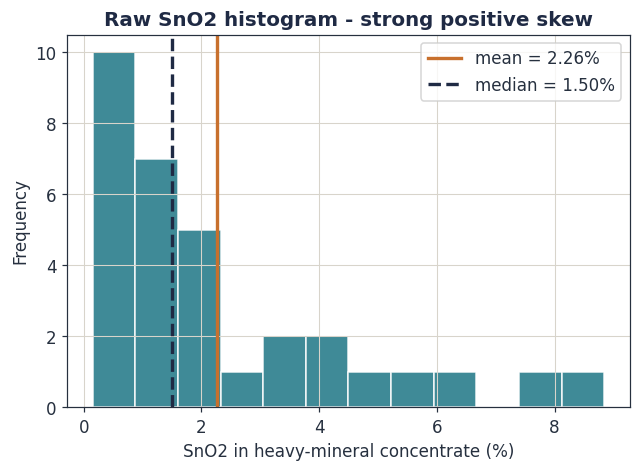
\includegraphics[width=0.72\textwidth]{../assets/figures/fig_histogram.png}
\caption{Histogram of the 32 Toro SnO$_2$ grades. The long right tail
drags the mean well above the median.}
\end{figure}

\section{The lognormal model of grade}

Grade is the product of many multiplicative geological processes, and
when independent random factors multiply, their product tends towards a
\textbf{lognormal} distribution: $Y=\ln Z \sim \mathcal{N}(\mu,\sigma^2)$.
The lognormal model explains the mean-median gap exactly:

\begin{eqbox}
\[ \operatorname{median}(Z)=e^{\mu},\qquad
   \mathbb{E}[Z]=e^{\,\mu+\sigma^2/2},\qquad
   \operatorname{Var}(Z)=(e^{\sigma^2}-1)e^{\,2\mu+\sigma^2} \tag{3.6}\]
\end{eqbox}

Because $\sigma^2/2>0$, the mean always exceeds the median. The
diagnostic tools follow: the log-transform should symmetrise the
histogram, and the lognormal probability plot should straighten the
ordered log-grades. For Toro, the log-transform collapses skewness from
$+1.48$ to $-0.09$ --- the grade is, to a good approximation, lognormal.

\begin{pitbox}[Never back-transform a kriged log-grade naively]
$\mathbb{E}[e^{Y}]\neq e^{\mathbb{E}[Y]}$: exponentiating a kriged
log-grade does not give the kriged grade, and the error is a systematic
bias. The safe default (Module 5) is to estimate in original units with
ordinary kriging after a sensible top-cut.
\end{pitbox}

\section{Clustered sampling and declustering}

Geologists drill where they expect grade, so high-grade ground is
over-sampled and the naive mean \emph{overstates} the deposit.
Declustering replaces the equal-weight mean with a weighted mean in which
each weight reflects the area a sample represents:

\begin{eqbox}
\[ \bar{z}_{\,dc} = \sum_{i=1}^{n} w_i\,z_i,
   \qquad \sum_{i=1}^{n} w_i = 1 \tag{3.7}\]
\end{eqbox}

In \emph{cell declustering}, a grid is laid over the data; each occupied
cell gets an equal share of weight, split among the samples inside it.
The Toro sampling is markedly clustered --- most of the 26 pits lie in
the Bishiwai and Yadabongo drainages, with only a handful at Kadade ---
so the naive mean of 2.27\% is biased towards Bishiwai.

\section{Outliers and the top-cut decision}

In a skewed dataset a few extreme values exert leverage far beyond their
number: the single 8.84\% Toro value contributes about 12\% of the summed
grade. \textbf{Top-cutting} resets values above a chosen cap to the cap.
The cap is documented judgement, informed by the probability-plot break,
the cumulative curve, and the metal-at-risk in the top one or two
samples. Toro's 97.5th percentile is 7.87\%, and a cap of 7--8\% removes
the leverage of the two highest values while discarding very little real
metal. Whatever cap is chosen must be stated, justified and its effect on
contained metal disclosed --- an undisclosed top-cut is a reporting
failure under every code.

\begin{figure}[h]\centering
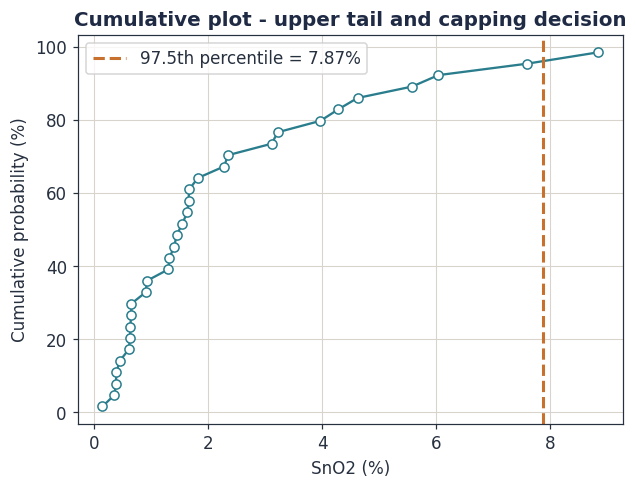
\includegraphics[width=0.66\textwidth]{../assets/figures/fig_cumprob.png}
\caption{Cumulative probability plot. The top two samples sit above a
visible inflection near 7.9\% SnO$_2$.}
\end{figure}

\section{Compositing: putting samples on equal support}

Statistics implicitly assume comparable data, but a 0.5 m drill interval
and a 2 m interval are different \textbf{supports} (the size, shape and
orientation a grade refers to). Compositing combines raw samples into
regular intervals of common support, length-weighted:

\begin{eqbox}
\[ z_{\text{comp}} = \frac{\sum_{i} \ell_i\, z_i}{\sum_{i} \ell_i}
   \tag{3.8}\]
\end{eqbox}

Composited grades scatter less than the raw samples they are built from
--- the first appearance of the \textbf{support effect}, formalised by
the volume-variance relationship in Module 6.

\begin{torobox}[Toro and the missing thickness]
The Module 2 audit composited Toro layer samples with a simple mean only
because the field logs do not consistently record sampled thickness. Equation
(3.8) shows why that is a real compromise: without $\ell_i$, a thin rich
gravel stringer and a thick lean one are averaged as equals. Recording
the sampled interval on every future pit is a prerequisite for a correct
composite.
\end{torobox}

\section{Domains and the decision of stationarity}

Every estimation method assumes that the pooled data belong to one
population --- that grade behaves consistently across the volume estimated.
That assumption is \textbf{stationarity}.

\begin{defbox}[Stationarity and the domain]
\textbf{Stationarity} is the assumption that the statistical properties
of grade --- mean, variance, spatial continuity --- do not depend on
absolute position within the volume considered. A \textbf{domain} is a
volume of rock within which stationarity can reasonably be assumed: one
mineralisation style, one grade population, one set of geological
controls.
\end{defbox}

Stationarity is not provable; it is, in Journel's phrase, a
\emph{decision}, defended by geological reasoning and supported by
statistics: side-by-side histograms, box plots, and \textbf{contact
analysis} (grade against distance across a proposed boundary --- a step
is a hard boundary, a gradient is a soft one).

\begin{pitbox}[The cardinal sin: pooling across domains]
If two genuinely different populations are pooled, the result is wrong
everywhere. A high-grade vein pooled with its low-grade halo produces a
variogram that describes neither and a kriging that bleeds vein grade
into waste. At Toro the non-negotiable boundary is between the
\textbf{alluvial} and \textbf{primary} targets: different rocks,
different grade units (g/m$^3$ vs \% Sn), different geometries and
different populations. They must be estimated as separate domains.
\end{pitbox}

Within the alluvial target, each drainage (Bishiwai, Yadabongo, Kadade)
is geologically a separate sediment-transport system. Present data
cannot resolve whether they are one statistical population or three, so
the conservative working decision is to carry them as sub-domains and
revisit once drilling adds data.

\section{Worked example: EDA on the Toro grades in Python}

\begin{lstlisting}
import numpy as np, pandas as pd
from scipy import stats

fs = pd.read_csv("data/toro_field_samples.csv")
z  = fs["SnO2"].values

mean   = z.mean()       # 2.27
median = np.median(z)   # 1.50
sd     = z.std(ddof=1)  # 2.21  (Bessel n-1)
cv     = sd / mean      # 0.98
skew   = stats.skew(z)  # +1.48

# lognormal test: log-transform should symmetrise
lz = np.log(z)
print(stats.skew(lz))   # -0.09  approximately symmetric

# metal at risk in the top two of 32 samples
top2 = np.sort(z)[-2:].sum() / z.sum() * 100
print(f"top 2 samples carry {top2:.0f}% of summed grade")  # 23%
\end{lstlisting}

Two samples out of 32 --- 6\% of the data --- carry 23\% of the summed
grade. That concentration of leverage is exactly what capping is designed
to control, and exactly what the codes require you to disclose.

\vspace{4pt}{\color{line}\hrule}\vspace{4pt}
{\small\itshape Module 3 of the Toro Resource Estimation course. Next:
Module 4, Spatial Continuity and Variography.}

\end{document}
